
% influences ***********
% Revisar aqui
% As Figuras \ref{fig:influence_sla}--\ref{fig:influence_avg_latency} apresentam uma análise de sensibilidade dos fatores (Algoritmo, Carga de trabalho e Disponibilidade de Nuvem) sobre cada métrica de resposta avaliada. Em cada gráfico, é mostrada a porcentagem de influência de cada fator isolado e das interações entre fatores, de acordo com um modelo de efeitos.


\begin{figure}[ht!]
    \centering
    \footnotesize

    % Latency SLA Violations
    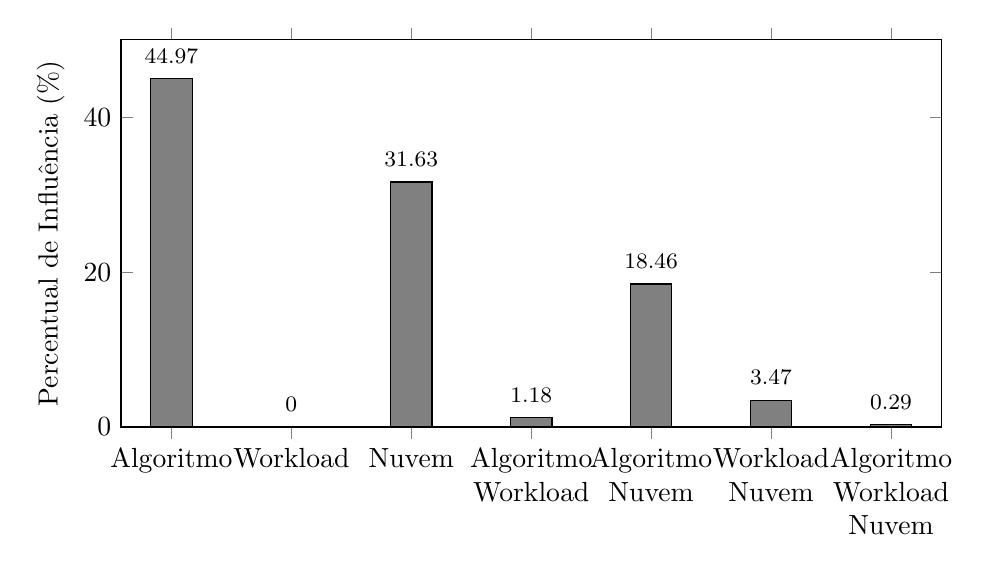
\begin{tikzpicture}
        \begin{axis}[
            ybar,
            symbolic x coords={Algoritmo, Workload, Nuvem, {Algoritmo\\Workload}, {Algoritmo\\Nuvem}, {Workload\\Nuvem}, {Algoritmo\\Workload\\Nuvem}},
            xtick=data,
            ymin=0,
            ymax=50,
            ylabel={Percentual de Influência (\%)},
            bar width=15pt,
            enlarge x limits=0.07,
            nodes near coords,
            every node near coord/.append style={font=\footnotesize, yshift=2pt},
            xticklabel style={align=center},
            width=12cm,
            height=6.5cm
        ]
        \addplot[ybar, fill=black!50, draw=black] coordinates {
            (Algoritmo, 44.97)
            (Workload, 0.00)
            (Nuvem, 31.63)
            ({Algoritmo\\Workload}, 1.18)
            ({Algoritmo\\Nuvem}, 18.46)
            ({Workload\\Nuvem}, 3.47)
            ({Algoritmo\\Workload\\Nuvem}, 0.29)
        };
        \end{axis}
    \end{tikzpicture}
    \caption{Influência de cada fator nas Violações de SLA de Latência}
    \label{fig:influence_sla}
\end{figure}

As figuras a seguir apresentam o nível de influência dos algoritmos, workload e da nuvem de maneira individual e em conjunto, sobre cada resultado analisado anteriormente. A Figura \ref{fig:influence_sla} refere-se às violações de SLA de latência. Verifica-se que o fator Algoritmo foi o mais influente, explicando cerca de 44,97\% da variação observada no número de violações de prazos. Isso significa que a escolha do algoritmo de alocação (SMMS, Thea ou EDF) tem impacto dominante na quantidade de deadlines perdidos, consistente com o fato de o SMMS ter apresentado bem menos violações que os outros. O segundo fator de maior influência é a presença da Nuvem, com aproximadamente 31,63\%. Ou seja, habilitar ou não recursos de nuvem afeta significativamente o cumprimento dos prazos (por exemplo, vimos que, para certos algoritmos, a ativação da nuvem pode aumentar as violações devido à maior latência de comunicação). Há também uma contribuição notável da interação Algoritmo\&Nuvem (cerca de 18,46\%): isso indica que o efeito da nuvem sobre as violações de SLA depende do algoritmo em uso. 

Na prática, cada algoritmo reagiu de forma diferente à disponibilidade de nuvem, o Thea teve um grande aumento de violações quando a nuvem estava ativada, enquanto o SMMS sofreu um aumento bem menor, e essa dependência se reflete no termo de interação. Já o fator \textit{Workload} (carga de trabalho) isolado teve influência praticamente nula (0\%), sugerindo que, no conjunto dos experimentos, a diferença entre carga baixa e alta não altera diretamente o número de violações de forma consistente. Esse resultado pode parecer contraintuitivo, mas explica-se porque o impacto da carga aparece principalmente combinado a outros fatores: por exemplo, carga alta só gera muitas violações quando a nuvem não está disponível e dependendo do algoritmo (o que se traduz nos termos de interação, não no efeito principal da carga por si só).


\begin{figure}[ht!]
    \centering
    \footnotesize

    % Average Latency
    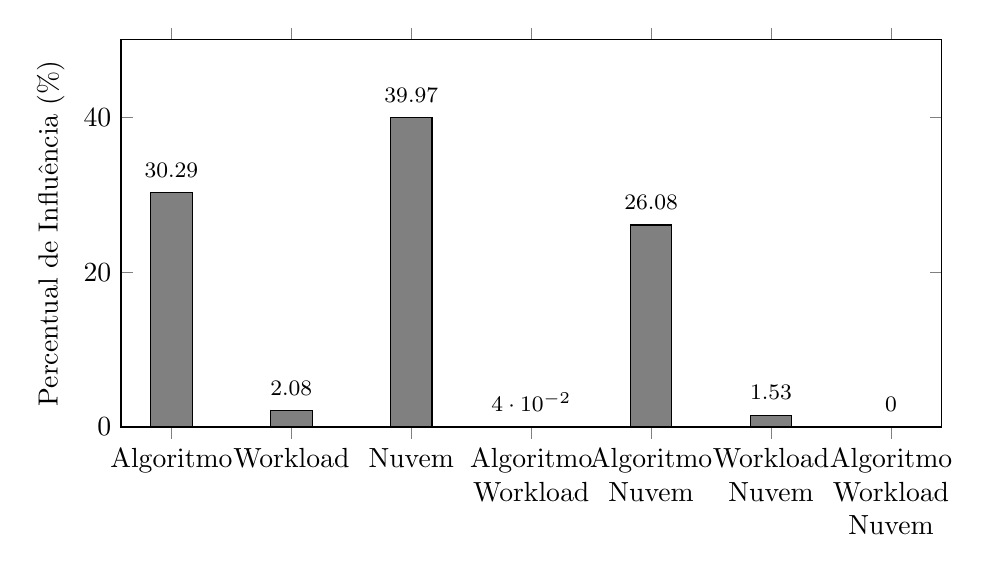
\begin{tikzpicture}
        \begin{axis}[
            ybar,
            symbolic x coords={Algoritmo, Workload, Nuvem, {Algoritmo\\Workload}, {Algoritmo\\Nuvem}, {Workload\\Nuvem}, {Algoritmo\\Workload\\Nuvem}},
            xtick=data,
            ymin=0,
            ymax=50,
            ylabel={Percentual de Influência (\%)},
            bar width=15pt,
            enlarge x limits=0.07,
            nodes near coords,
            every node near coord/.append style={font=\footnotesize, yshift=2pt},
            xticklabel style={align=center},
            width=12cm,
            height=6.5cm
        ]
        \addplot[ybar, fill=black!50, draw=black] coordinates {
            (Algoritmo, 30.29)
            (Workload, 2.08)
            (Nuvem, 39.97)
            ({Algoritmo\\Workload}, 0.04)
            ({Algoritmo\\Nuvem}, 26.08)
            ({Workload\\Nuvem}, 1.53)
            ({Algoritmo\\Workload\\Nuvem}, 0.00)
        };
        \end{axis}
    \end{tikzpicture}
    \caption{Influência de cada fator na Latência Média}
    \label{fig:influence_avg_latency}
\end{figure}


Na Figura \ref{fig:influence_avg_latency}, vemos os fatores influenciando a latência média das requisições. O fator Nuvem é o mais significativo, respondendo por cerca de 39,97\% da variação na latência média. Esse alto percentual confirma que enviar aplicações para um servidor remoto (nuvem) eleva substancialmente os tempos de resposta médios, dominando o comportamento dessa métrica. Em seguida, o fator Algoritmo contribui com aproximadamente 30,29\% da variação de latência. Ou seja, a política de alocação adotada também impacta bastante o tempo médio de atendimento, por exemplo, o SMMS tende a minimizar latências ao preferir processamento local, enquanto o Thea introduz mais latência com um \textit{offloading} agressivo para a nuvem. Novamente, observa-se um efeito importante da interação Algoritmo\&Nuvem (cerca de 26,08\%): isso significa que o aumento de latência devido à nuvem varia conforme o algoritmo (como visto, o prejuízo de latência com nuvem foi enorme no Thea, moderado no EDF e relativamente baixo no SMMS). A Carga de trabalho mais uma vez aparece com influência direta muito pequena (apenas 2,08\%), indicando que o mero aumento do volume de requisições (de Low para High) não eleva drasticamente a latência média se considerado isoladamente, o efeito da carga manifesta-se principalmente através da combinação com a falta de nuvem ou com certas decisões do algoritmo (por exemplo, sob alta carga alguns algoritmos podem passar a usar mais a nuvem, elevando latências, mas isso está capturado no termo de interação Algoritmo\&Carga e Algoritmo\&Nuvem, não no efeito puro da carga).


\begin{figure}[ht!]
    \centering
    \footnotesize

    % Drop SLA Violations
    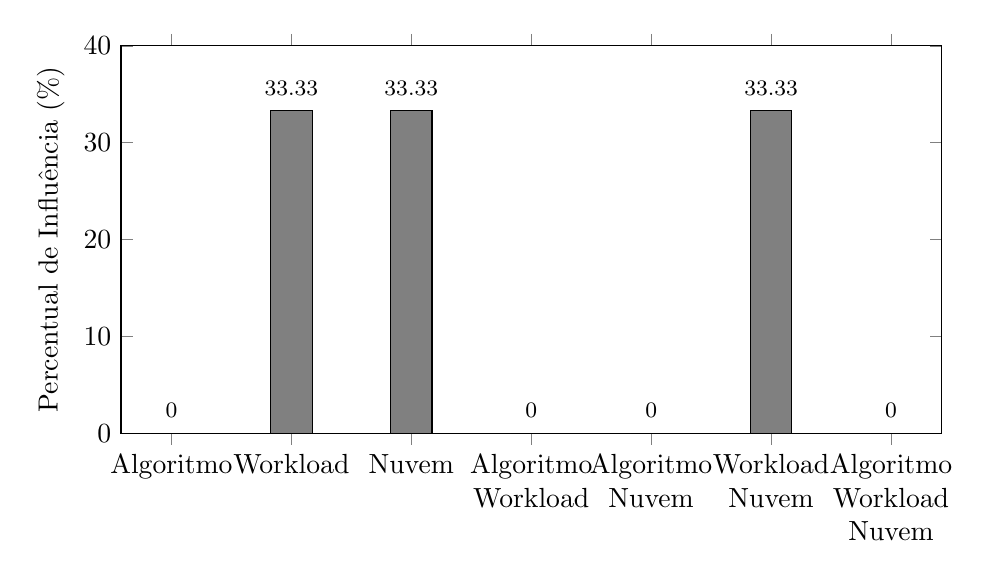
\begin{tikzpicture}
        \begin{axis}[
            ybar,
            symbolic x coords={Algoritmo, Workload, Nuvem, {Algoritmo\\Workload}, {Algoritmo\\Nuvem}, {Workload\\Nuvem}, {Algoritmo\\Workload\\Nuvem}},
            xtick=data,
            ymin=0,
            ymax=40,
            ylabel={Percentual de Influência (\%)},
            bar width=15pt,
            enlarge x limits=0.07,
            nodes near coords,
            every node near coord/.append style={font=\footnotesize, yshift=2pt},
            xticklabel style={align=center},
            width=12cm,
            height=6.5cm
        ]
        \addplot[ybar, fill=black!50, draw=black] coordinates {
            (Algoritmo, 0.00)
            (Workload, 33.33)
            (Nuvem, 33.33)
            ({Algoritmo\\Workload}, 0.00)
            ({Algoritmo\\Nuvem}, 0.00)
            ({Workload\\Nuvem}, 33.33)
            ({Algoritmo\\Workload\\Nuvem}, 0.00)
        };
        \end{axis}
    \end{tikzpicture}
    \caption{Influência de cada fator nas Violações de SLA por Drop}
    \label{fig:influence_drop}
\end{figure}

A Figura \ref{fig:influence_drop} mostra a análise para as violações de SLA por drop (serviços não alocados). Aqui, fica evidente que o Algoritmo não teve influência direta alguma (0\%) sobre essa métrica, enquanto os fatores Carga de trabalho, Nuvem e a interação Carga\&Nuvem dividem igualmente a influência (aproximadamente 33,33\% cada). Essa distribuição indica que os drops só ocorreram em uma condição muito específica, justamente quando a carga era alta e a nuvem estava indisponível. Nesse caso, todos os algoritmos acabaram apresentando um número semelhante de serviços não alocados (conforme vimos, \textasciitilde1 drop em High Off), de modo que a diferença entre SMMS, Thea ou EDF não afetou a ocorrência de drops. Em contraste, a combinação de alta carga com ausência de nuvem foi necessária para a aparição de drops, o que explica por que a interação entre carga e nuvem, junto com os efeitos individuais de cada um, respondem por 100\% da variação. Em outras palavras, se a carga não estiver elevada ou se a nuvem estiver disponível, nenhum drop aconteceu nos experimentos (0\% de violações por drop); somente quando ambas as condições se juntam é que observamos violação de SLA por falta de alocação.


\begin{figure}[ht!]
    \centering
    \footnotesize

    % Requests
    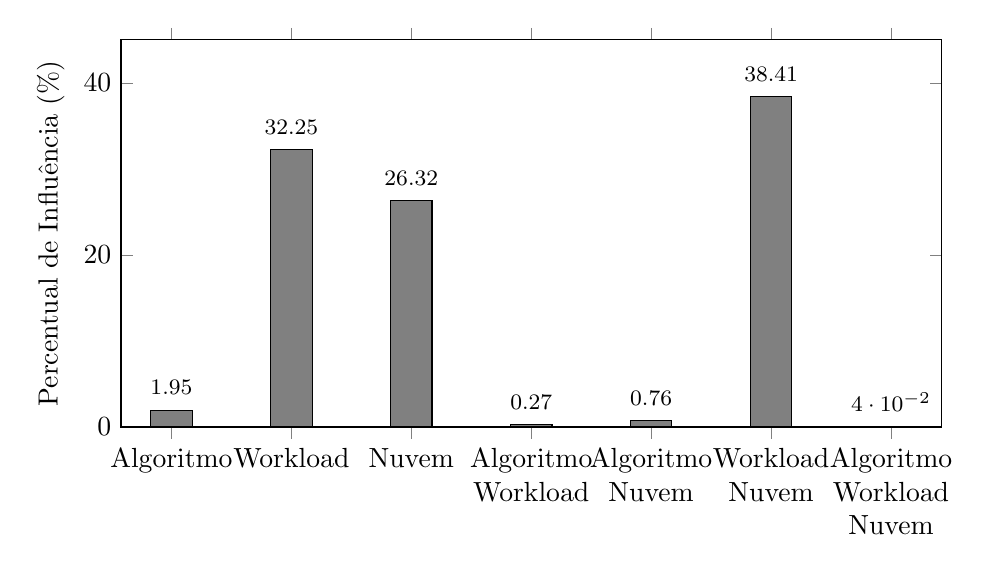
\begin{tikzpicture}
        \begin{axis}[
            ybar,
            symbolic x coords={Algoritmo, Workload, Nuvem, {Algoritmo\\Workload}, {Algoritmo\\Nuvem}, {Workload\\Nuvem}, {Algoritmo\\Workload\\Nuvem}},
            xtick=data,
            ymin=0,
            ymax=45,
            ylabel={Percentual de Influência (\%)},
            bar width=15pt,
            enlarge x limits=0.07,
            nodes near coords,
            every node near coord/.append style={font=\footnotesize, yshift=2pt},
            xticklabel style={align=center},
            width=12cm,
            height=6.5cm
        ]
        \addplot[ybar, fill=black!50, draw=black] coordinates {
            (Algoritmo, 1.95)
            (Workload, 32.25)
            (Nuvem, 26.32)
            ({Algoritmo\\Workload}, 0.27)
            ({Algoritmo\\Nuvem}, 0.76)
            ({Workload\\Nuvem}, 38.41)
            ({Algoritmo\\Workload\\Nuvem}, 0.04)
        };
        \end{axis}
    \end{tikzpicture}
    \caption{Influência de cada fator nas solicitações}
    \label{fig:influence_requests}
\end{figure}
    

A Figura \ref{fig:influence_requests} refere-se ao número de requisições processadas com sucesso. Os resultados mostram que a interação Carga\&Nuvem é o fator mais influente, explicando cerca de 38,41\% da variação no total de requests atendidos, seguida pelo efeito isolado da Carga de trabalho (32,25\%) e da Nuvem (26,32\%). Isso reflete o fato de que o único cenário em que houve diferença significativa no número de requisições atendidas foi sob carga alta sem nuvem, justamente a combinação desses dois fatores. Em todas as demais configurações (carga baixa com/sem nuvem, carga alta com nuvem), a maior parte das requisições foram atendidas, independente do algoritmo, resultando em pouca variação entre esses casos. Por isso, a interação de carga alta e nuvem off domina a estatística.

O Algoritmo, por outro lado, teve influência mínima (apenas 1,95\%): isto significa que SMMS, Thea e EDF não diferiram significativamente em termos de \textit{throughput} ou capacidade de atender requisições quando submetidos às mesmas condições de carga e recursos. Todos os três algoritmos conseguiram atender quantidades equivalentes de solicitações, limitados principalmente pelos recursos disponíveis (borda e nuvem ou apenas borda) e pelo nível de demanda, e não pela eficiência intrínseca de cada algoritmo nesse quesito.


\begin{figure}[ht!]
    \centering
    \footnotesize

    % Success Rate
    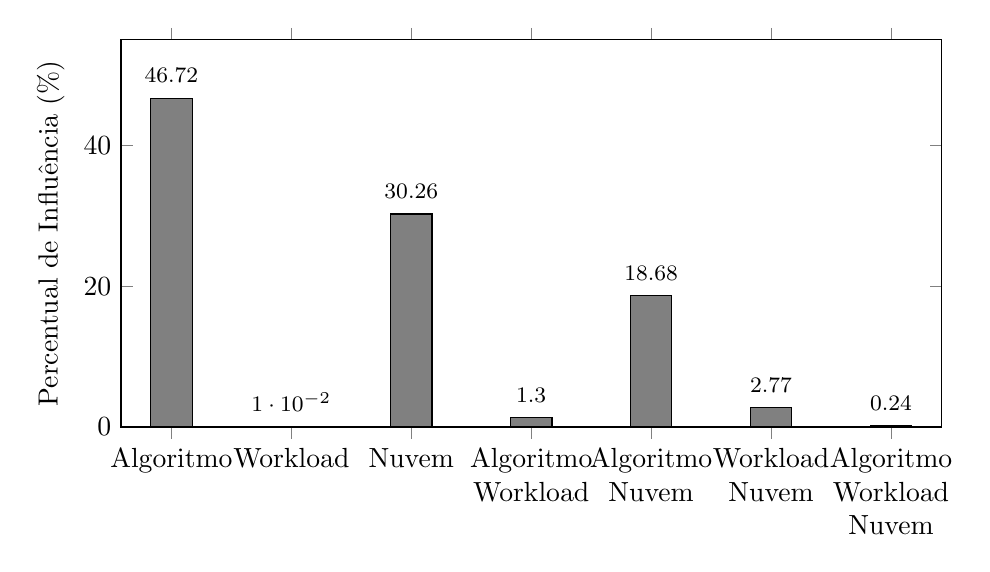
\begin{tikzpicture}
        \begin{axis}[
            ybar,
            symbolic x coords={Algoritmo, Workload, Nuvem, {Algoritmo\\Workload}, {Algoritmo\\Nuvem}, {Workload\\Nuvem}, {Algoritmo\\Workload\\Nuvem}},
            xtick=data,
            ymin=0,
            ymax=55,
            ylabel={Percentual de Influência (\%)},
            bar width=15pt,
            enlarge x limits=0.07,
            nodes near coords,
            every node near coord/.append style={font=\footnotesize, yshift=2pt},
            xticklabel style={align=center},
            width=12cm,
            height=6.5cm
        ]
        \addplot[ybar, fill=black!50, draw=black] coordinates {
            (Algoritmo, 46.72)
            (Workload, 0.01)
            (Nuvem, 30.26)
            ({Algoritmo\\Workload}, 1.30)
            ({Algoritmo\\Nuvem}, 18.68)
            ({Workload\\Nuvem}, 2.77)
            ({Algoritmo\\Workload\\Nuvem}, 0.24)
        };
        \end{axis}
    \end{tikzpicture}
    \caption{Influência de cada fator na taxa de sucesso}
    \label{fig:influence_success}
\end{figure}

A Figura \ref{fig:influence_success} mostra os fatores de influência para a taxa de sucesso no cumprimento dos SLAs. Como esperado, os resultados são praticamente o espelho das violações de latência (já que a taxa de sucesso se trata de 100\% subtraído do percentual de violações). O Algoritmo responde por cerca de 46,72\% da variação na taxa de sucesso, sendo o fator mais importante, o que reforça que a escolha do SMMS em vez de Thea, por exemplo, eleva drasticamente o percentual de requisições dentro do prazo. A Nuvem contribui com cerca de 30,26\%, consistente com o efeito que a disponibilidade de nuvem altera as latências (a presença da nuvem, dependendo do caso, pode tanto permitir atender mais requisições quanto introduzir atrasos que prejudicam o sucesso temporal).

A interação Algoritmo\&Nuvem aparece com 18,68\% de influência, novamente indicando que o impacto da nuvem na taxa de sucesso varia conforme o algoritmo, p.ex., o Thea teve uma queda enorme de sucesso com a nuvem ligada, enquanto o SMMS conseguiu manter sucesso alto, o que produz um termo de interação significativo. Os demais fatores têm efeitos pequenos: a Carga de trabalho sozinha praticamente não afeta a taxa de sucesso (0,01\%), assim como outras interações de ordem superior são negligenciáveis. Em resumo, para garantir alta proporção de requisições dentro do SLA, o mais determinante é empregar um algoritmo eficaz (como o SMMS) e dispor de recursos de nuvem quando possível, sabendo que algoritmos distintos tiram proveito (ou não) da nuvem de maneiras distintas.


% \begin{figure}[ht!]
%     \centering
%     \footnotesize

%     % Power Consumption
%     \begin{tikzpicture}
%         \begin{axis}[
%             ybar,
%             symbolic x coords={Algoritmo, Workload, Nuvem, {Algoritmo\\Workload}, {Algoritmo\\Nuvem}, {Workload\\Nuvem}, {Algoritmo\\Workload\\Nuvem}},
%             xtick=data,
%             ymin=0,
%             ymax=50,
%             ylabel={Percentual de Influência (\%)},
%             bar width=15pt,
%             enlarge x limits=0.07,
%             nodes near coords,
%             every node near coord/.append style={font=\footnotesize, yshift=2pt},
%             xticklabel style={align=center},
%             width=12cm,
%             height=6.5cm
%         ]
%         \addplot[ybar, fill=black!50, draw=black] coordinates {
%             (Algoritmo, 37.87)
%             (Workload, 7.83)
%             (Nuvem, 41.70)
%             ({Algoritmo\\Workload}, 12.34)
%             ({Algoritmo\\Nuvem}, 0.02)
%             ({Workload\\Nuvem}, 0.12)
%             ({Algoritmo\\Workload\\Nuvem}, 0.13)
%         };
%         \end{axis}
%     \end{tikzpicture}
%     \caption{Influence of each factor on Power Consumption}
%     \label{fig:influence_power}
% \end{figure}

% A Figura \ref{fig:influence_power} exibe a influência dos fatores sobre o consumo de potência da infraestrutura (borda e nuvem). Os dois principais fatores são a Nuvem, responsável por aproximadamente 41,70\% da variação, e o Algoritmo, contribuindo com cerca de 37,87\%. O efeito da nuvem é significativo porque ativar um servidor de nuvem introduz um consumo de energia adicional considerável, mesmo se o servidor estiver ocioso, há um custo base, e quando ele processa requisições, adiciona consumo acima do que as bordas sozinhas consumiriam. Já a influência do algoritmo indica que as políticas de alocação conseguem impactar o uso energético: por exemplo, o SMMS geralmente consumiu menos energia que o Thea, pois faz um uso mais eficiente dos recursos (consolidando serviços em menos servidores quando possível e evitando ligações desnecessárias à nuvem), enquanto o Thea pode manter mais servidores ativos ou usar a nuvem de forma menos eficiente energeticamente. O fator Carga de trabalho teve impacto menor, cerca de 7,83\%, o que faz sentido, cargas mais altas aumentam o uso dos servidores e, portanto, o consumo, mas esse efeito é relativamente linear e inferior às diferenças causadas por ter ou não um datacenter de nuvem no circuito.

% Vale destacar o termo de interação Algoritmo\&Carga (12,34\%), indicando que alguns algoritmos escalam o consumo de energia de forma diferente conforme a demanda cresce. Por exemplo, o Thea pode acionar recursos de nuvem (que têm custo fixo alto) já em cargas moderadas, enquanto o SMMS talvez só faça isso em cargas muito altas, o que faz o consumo do Thea crescer mais rapidamente com o aumento da carga. Já a interação Algoritmo\&Nuvem foi praticamente nula (0,02\%), sugerindo que todos os algoritmos, ao terem a nuvem ligada, incorrem num acréscimo de consumo relativamente semelhante (o diferencial está mais em quanto cada algoritmo utiliza a infraestrutura em geral, e não no custo fixo da nuvem em si). Em síntese, o SMMS conseguiu reduzir o consumo energético médio da infraestrutura em comparação com o Thea, resultado refletido nesses valores de influência.


% \begin{figure}[ht!]
%     \centering
%     \footnotesize

%     % Servers Usage
%     \begin{tikzpicture}
%         \begin{axis}[
%             ybar,
%             symbolic x coords={Algoritmo, Workload, Nuvem, {Algoritmo\\Workload}, {Algoritmo\\Nuvem}, {Workload\\Nuvem}, {Algoritmo\\Workload\\Nuvem}},
%             xtick=data,
%             ymin=0,
%             ymax=60,
%             ylabel={Percentual de Influência (\%)},
%             bar width=15pt,
%             enlarge x limits=0.07,
%             nodes near coords,
%             every node near coord/.append style={font=\footnotesize, yshift=2pt},
%             xticklabel style={align=center},
%             width=12cm,
%             height=6.5cm
%         ]
%         \addplot[ybar, fill=black!50, draw=black] coordinates {
%             (Algoritmo, 52.50)
%             (Workload, 20.92)
%             (Nuvem, 13.60)
%             ({Algoritmo\\Workload}, 11.74)
%             ({Algoritmo\\Nuvem}, 0.74)
%             ({Workload\\Nuvem}, 0.49)
%             ({Algoritmo\\Workload\\Nuvem}, 0.01)
%         };
%         \end{axis}
%     \end{tikzpicture}
%     \caption{Influence of each factor on Servers Usage}
%     \label{fig:influence_servers}
% \end{figure}

% Por fim, a Figura \ref{fig:influence_servers} mostra a influência sobre o uso percentual dos servidores (isto é, o grau de utilização da capacidade de processamento disponível). O fator Algoritmo se destaca fortemente, explicando cerca de 52,50\% da variação no uso dos servidores. Isso significa que cada algoritmo gerencia a carga de forma distinta em termos de ocupação dos servidores: o SMMS tende a utilizar menos a capacidade total (mantendo folga nos servidores), enquanto o Thea e o EDF usam porcentagens maiores da capacidade ou de forma menos equilibrada. Esse comportamento do SMMS, de não sobrecarregar completamente os servidores, condiz com sua estratégia de alocação distribuída e preventiva, evitando saturação para garantir baixa latência. Já o Thea, por exemplo, pode subutilizar deliberadamente as bordas (offloading para a nuvem mesmo com capacidade local livre) ou, em outros cenários, pode sobrecarregar servidores locais até o limite antes de recorrer à nuvem, dependendo de seus objetivos de otimização, de qualquer forma, o resultado é um perfil de uso bem diferente do SMMS. O nível de Carga de trabalho em si responde por cerca de 20,92\% da variação no uso: naturalmente, carga alta leva a um uso mais intenso dos servidores em comparação à carga baixa, mas esse efeito isolado é menor do que as discrepâncias de utilização geradas pelas diferentes políticas. A presença da Nuvem contribui com cerca de 13,60\%, a disponibilidade de nuvem tende a reduzir a média de uso dos servidores de borda, pois parte da carga pode ser transferida para a nuvem (espalhando o uso total por mais máquinas), embora em alguns casos a nuvem também permita processar mais requisições totais, elevando um pouco o uso global. Os termos de interação têm influência moderada: por exemplo, Algoritmo\&Carga representa \textasciitilde11,74\%, indicando que o impacto de aumentar a carga depende do algoritmo (alguns algoritmos degradam a distribuição de carga mais do que outros quando sobrecarregados). No geral, a análise confirma que o SMMS promove um uso mais equilibrado e parcimonioso dos recursos de borda, evitando tanto ociosidade excessiva quanto saturação, o que explica por que obteve simultaneamente baixa latência e menor consumo de energia.

    

Os resultados quantitativos finais são resumidos na Tabela \ref{tab:final_results_comparison}, que apresenta os valores médios e desvios padrão de cada métrica para todas as combinações de algoritmo, carga e nuvem avaliadas. Observa-se que, em todos os cenários, o SMMS iguala ou supera o Thea em desempenho. Especificamente, em termos de violações de SLA de latência, o SMMS apresenta números drasticamente menores. Por exemplo, com carga baixa e nuvem (Low On), o SMMS teve em média 17,3 violações contra 274,1 do Thea; com carga alta e nuvem (High On), 69,6 vs 302,0; e assim por diante. Em média global, o SMMS reduziu o número de deadlines perdidos em cerca de 84\% em relação ao Thea. Além disso, o SMMS eliminou praticamente todas as violações de SLA por drop, ambos SMMS e Thea não tiveram qualquer drop na maioria dos cenários, e mesmo no pior caso (High Off) houve apenas 1 drop em cada, mas note-se que esse 1 drop para o SMMS não afetou seu SLA de latência tanto quanto as decisões do Thea afetaram o dele.

Com relação à latência média, o SMMS alcançou tempos significativamente menores: aproximadamente 20–60 ms dependendo do cenário, enquanto o Thea variou de \textasciitilde28 ms (quando forçado a utilizar apenas a borda) até 206 ms (com acesso à nuvem e sob alta carga). Portanto, o SMMS conseguiu respostas mais rápidas, chegando a ser 3 a 4 vezes mais veloz que o Thea nos cenários com nuvem. Em resumo, os dados da Tabela \ref{tab:final_results_comparison} destacam a vantagem abrangente do SMMS: ele mantém melhor conformidade de SLA (menos violações e nenhum drop) e melhora a latência para os usuários em comparação com uma solução do estado da arte, Thea. O algoritmo EDF, incluído como referência, apresenta desempenho intermediário nas métricas de SLA e consumo, ficando consistentemente atrás do SMMS e em alguns casos próximo ou ligeiramente à frente do Thea, mas sem atingir o equilíbrio de desempenho e eficiência proporcionado pela abordagem multiagente do SMMS.

\begin{table}[ht!]
\footnotesize
\setlength{\tabcolsep}{3pt}
\renewcommand{\arraystretch}{1.15}
\caption{Métricas de desempenho (violações de latência, drops, latência média e taxa de sucesso) para SMMS, Thea e EDF sob diferentes condições de carga e Nuvem.}
\label{tab:final_results_comparison}
\begin{center}
\begin{tabular}{cccc|cc|cc|cc|cc}
\hline
Algo & Load & Nuvem & & \multicolumn{2}{c|}{Viol. Latência} & \multicolumn{2}{c|}{\textit{Drops}} & \multicolumn{2}{c|}{Latência Média} & \multicolumn{2}{c}{Taxa de Sucesso (\%)} \\\cline{5-12}
     &      &       & & mean & std & mean & std & mean & std & mean & std \\ \hline
SMMS & Low  & On    & & 17.3 & 27.9 & 0.0 & 0.0 & 20.0 & 0.0 & 95.0 & 0.0 \\
SMMS & Low  & Off   & & 17.3 & 27.9 & 0.0 & 0.0 & 20.0 & 0.0 & 95.0 & 0.0 \\
SMMS & High & On    & & 69.6 & 22.4 & 0.0 & 0.0 & 60.0 & 0.0 & 80.0 & 0.0 \\
SMMS & High & Off   & & 10.6 & 22.4 & 1.0 & 0.0 & 26.0 & 0.0 & 96.0 & 0.0 \\ \hline
Thea & Low  & On    & & 274.1 & 20.0 & 0.0 & 0.0 & 170.97 & 9.6 & 14.82 & 3.72 \\
Thea & Low  & Off   & & 106.9 & 36.7 & 0.0 & 0.0 & 28.7 & 3.0 & 66.89 & 11.45 \\
Thea & High & On    & & 302.0 & 8.5 & 0.0 & 0.0 & 205.98 & 0.3 & 8.72 & 2.28 \\
Thea & High & Off   & & 28.1 & 47.7 & 1.0 & 0.0 & 28.4 & 1.3 & 90.0 & 17.0 \\ \hline
EDF  & Low  & On    & & 175.4 & 14.3 & 0.0 & 0.0 & 81.04 & 4.9 & 47.8 & 4.62 \\
EDF  & Low  & Off   & & 88.6 & 25.4 & 0.0 & 0.0 & 29.01 & 1.4 & 73.84 & 7.64 \\
EDF  & High & On    & & 230.5 & 9.6 & 0.0 & 0.0 & 136.69 & 3.5 & 31.75 & 2.93 \\
EDF  & High & Off   & & 75.3 & 43.3 & 0.9 & 0.7 & 29.61 & 2.8 & 73.88 & 16.42 \\ \hline
\end{tabular}
\end{center}
\end{table}

Além disso, em uma análise mais granularizada do comportamento dos algoritmos, notou-se que o Thea tende a se manter constantemente migrando serviços entre os servidores e, por vezes, pode ``demorar'' para realizar a alocação inicial de um dado serviço. Em contrapartida, a abordagem multiagente apresentada foca em mover os serviços para uma posição considerada ideal e migrá-los apenas se estritamente necessário. Ou seja, no SMMS os serviços são alocados mais rápido e raramente migrados (considerando cenários de curtos períodos de tempo). Isso pode estar associado ao impacto nas requisições atendidas por cada algoritmo, entre outros fatores.